\vspace*{-1mm}
The beam and machine conditions for the emittance growth studies were discussed extensively in Chapter~\ref{Ch:2018_setup} and are listed in Tables~\ref{tab:machine_beam_param_2018} and~\ref{tab:SPS_CC_main}. In principle the measurements were performed with four bunches at 270\,GeV with low intensity (3 $\times \mathrm{10^{10}}$ ppb) with linear chromaticity corrected to to $\sim$ 1. Only $\CC2$ was used, provied a vertical kick on the beam. In order to characterize the CC noise induced emittance growth, different levels of controlled noise were injected into their LLRF system and the bunch evolution was recorded for about 20-40 minutes (for each noise setting). Three "coasts" were carried out, since a new beam was injected every time the quality of the beam was seen to be degraded e.g. due to large emittance values. 

In this Chapter the measurements that were performed during the experiment and their analysis are presented. Section 


1. present brifly the parameters
2. injected rf noise
3. MD emittance growth overview. 
    - average from IN and OUT. As mentioned in CH4. vs time and vs noise level for all bunches. Not yet comparison with the theory. Probably you need to re-run this to make correctly the error propagation. 
    - 1 noise point was excluded
    - bunch length and longitudinal profiles and relative position from the wall current monitor.  unstable bunches.
    - bunch 2-3-4 longutidinally unstable.
    - intensity --> no losses.
4. bunch 1 comparison with the theory. dey/dt vs noise levels plots. Factor of 4-5 difference. 

Par 2: Section 5.1 .. blah blah

\section{CC voltage}\label{sec:CC_voltage_meas2018}
A reference measurement of the CC voltage was made before going into coast and is displayed in Fig ... . It was assumed that the voltage remained unchanged through the experiment. High uncertainty due to the coast at 270 GeV

\section{Injected RF noise}\label{sec:noisemeas2018}
\begin{sloppypar} % to fix \hbox too wide
 The injected noise was a mixture of amplitude and phase noise up to 10\,kHz, overlapping and primarily exciting the first betatron sideband at $\sim 8$\,kHz. The phase noise was always dominant. Figure~\ref{fig:example_PN_and_AN} dsiplays two example measurements of phase (left) and amplitude (right) noise acquired during the experiment with a sepctrum analyzer E5052B~\cite{E5052B_insight}. 
\end{sloppypar} 

 % Loaction for creating the figure: /cernbox/2020/injected_noise_MD5_2018
 \begin{figure}[!ht]
    \centering
    \begin{subfigure}[t]{0.45\textwidth}
        \centering
        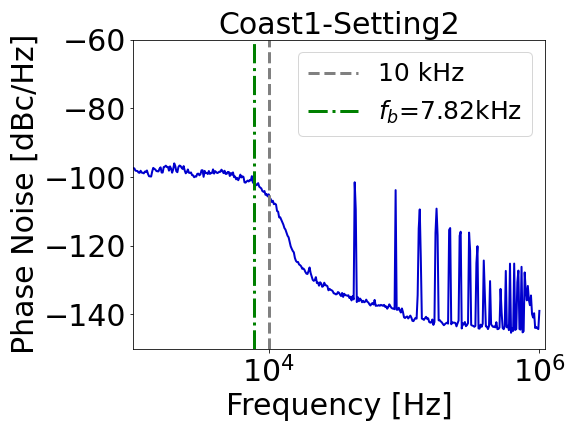
\includegraphics[width=1\textwidth]{images/Ch5/Measured_spectrum_MD5_Coast1-Setting2-PN.csv_no_psd.png}
        %\caption{$y=\sin(2 \pi f t),\ f=50$ Hz}
        %\label{fig:add_label_here}
    \end{subfigure}
    \hfill
    \begin{subfigure}[t]{0.45\textwidth}
        \centering
        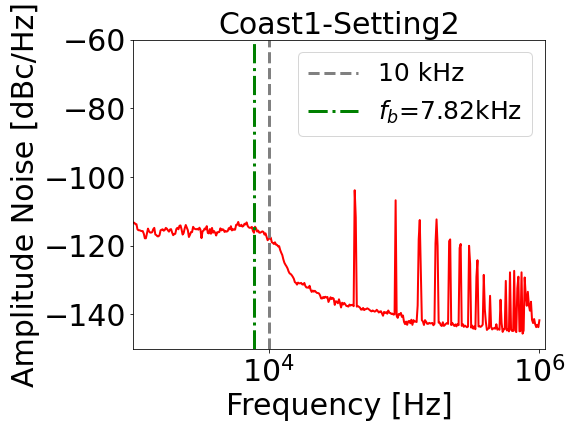
\includegraphics[width=1\textwidth]{images/Ch5/Measured_spectrum_MD5_Coast1-Setting2-AN.csv_no_psd.png}
        %\caption{Discrete Fourier transform}
        %\label{fig:add_label_here}
    \end{subfigure}
    \hfill
     \caption{Example phase (left) and amplitude (right) noise spectra measured with a spectrum analyzer E5052B during the emittance growth studies with CCs in SPS. The noise spread-out up to 10\,kHz (grey dashed line) exciting the first betatron sideband at $\sim$8\,kHz (green dashed line). The spikes at high frequencies correspond to the harmonics of the revolution frequency and are a result of the bunch crossing.} % bunch passage
     \label{fig:example_PN_and_AN}
\end{figure}

\begin{sloppypar} % to fix \hbox too wide
This spectrum analyzer provides a single sideband measurement (SSB), which is expressed as $10\log_{10}\mathcal{L}(f)$\,[dBc/Hz]. Its relation with the power spectral densities (PSDs) introduced in Eq.~\eqref{eq:dey_an} and Eq.~\eqref{eq:dey_pn} are given by $S_\Delta = 2\mathcal{L}(f)$~\cite{IEEE:4797525}, with $S_{\Delta A}$ in 1/Hz and $S_{\Delta\phi}$ in rad$^2$/Hz. A detailed discussion on the noise power measurements and their relation to the mathimatical defintion of the PSD is given in Chapter [tba].

As already mentioned above the injected noise was a combination of both phase and amplitude noise. Therefore, in order to make a meaningful comparison between the different noise levels the concept of effective phase noise is introduced. This is the phase noise level that would lead to
the same emittance growth as that from both phase and
amplitude noise. The noise levels mentioned in this Chapter correspond to the calculated effective phase noise.
% should I slightly change this paragraph? Too much copy paste from IPAC or it's ok?
\end{sloppypar} 

\subsection{Emittance growth measurements}\label{subsec:EmitGrowth_measurements}


 \section{Comparison with the theory}\label{sec:MD2018_vs_theory}


 \section{Conclusions and outlook}